%% LaTeX-Beamer template for KIT design
%% by Erik Burger, Christian Hammer
%% title picture by Klaus Krogmann
%%
%% version 2.1
%%
%% mostly compatible to KIT corporate design v2.0
%% http://intranet.kit.edu/gestaltungsrichtlinien.php
%%
%% Problems, bugs and comments to
%% burger@kit.edu

\documentclass[18pt]{beamer}
\usepackage[utf8x]{inputenc}
\usepackage{units}
\usepackage{booktabs}

%% CUSTOM
\usepackage{amsmath}
\usepackage{algpseudocode}

%% Definitions
\DeclareMathOperator{\div2}{div}
\renewcommand{\algorithmicrequire}{\textbf{Input:}}
\renewcommand{\algorithmicensure}{\textbf{Output:}}
\algnewcommand\algorithmicto{\textbf{to}}
\algrenewtext{For}[3]{\algorithmicfor\ $#1 \gets #2$ \algorithmicto\ $#3$ \algorithmicdo}
\algnewcommand\algorithmicod{\textbf{od}}
\algrenewtext{EndWhile}{\algorithmicod}
\algrenewtext{EndFor}{\algorithmicod}
%\AtBeginSection[]{%
%\begin{frame}<beamer> % do nothing in handouts
%    \frametitle{Überblick}
%    \tableofcontents[sectionstyle=show/shaded,
%    subsectionstyle=show/show/hide]
%\end{frame}
%}
%\AtBeginSubsection[]{%
%\begin{frame}<beamer> % do nothing in handouts
%    \frametitle{Überblick}
%    \tableofcontents[sectionstyle=show/shaded,
%    subsectionstyle=show/shaded/hide]
%\end{frame}
%}

%% SLIDE FORMAT

% use 'beamerthemekit' for standard 4:3 ratio
% for widescreen slides (16:9), use 'beamerthemekitwide'

\usepackage{templates/beamerthemekit}
%\usepackage{templates/beamerthemekitwide}

 %% TITLE PICTURE

 % if a custom picture is to be used on the title page, copy it into the 'logos'
 % directory, in the line below, replace 'mypicture' with the 
 % filename (without extension) and uncomment the following line
 % (picture proportions: 63 : 20 for standard, 169 : 40 for wide
 % *.eps format if you use latex+dvips+ps2pdf, 
 % *.jpg/*.png/*.pdf if you use pdflatex)


 \titleimage{banner}
 
 
%% Define some colors:
\definecolor{darkblue}{rgb}{0,0,.5}
\definecolor{darkgreen}{rgb}{0,.5,0}

 %% TITLE LOGO

 % for a custom logo on the front page, copy your file into the 'logos'
 % directory, insert the filename in the line below and uncomment it

\titlelogo{logo_150x150}
 
 % (*.eps format if you use latex+dvips+ps2pdf,
 % *.jpg/*.png/*.pdf if you use pdflatex)
 
 %% TikZ INTEGRATION
 
 % use these packages for PCM symbols and UML classes
 % \usepackage{templates/tikzkit}
 % \usepackage{templates/tikzuml}
 
 % the presentation starts here
 
\author{Dominik Muth - dominik.muth@student.kit.edu}
\institute{Institut f\"ur Informatik}


\title[Tutorium 8]{GBI Tutorium Nr. $2^5$}
\subtitle{Tutorium 8}
\date{12. Dezember 2012}

% Bibliography



\begin{document}

	%title page
	\begin{frame}
		\titlepage
	\end{frame}

	%table of contents
	\begin{frame}{Outline/Gliederung}
		\tableofcontents
	\end{frame}	
		
	
	
	\section{Wiederholung} 
	\begin{frame} {Wiederholung - Quiz}
		\begin{itemize}
			\item In Adjazenzmatrizen sind immer schneller als Adjazenzlisten, benötigen aber mehr Speicher.
			\only<2-> {\color{red}$X$}\\
			\color{black}
					
			\item Hat ein Knoten x keine Ausgehenden Kanten, so steht in der Wegematrix in der x. Zeile nur 0en.
			\only<3-> {\color{red}$X$}\\
			\color{black}
	
			\item Über Matrizenmultiplikation und addition lässt sich eine Wegematrix konstruieren.
			\only<4-> {\color{darkgreen}$\surd$}\\
			\color{black}
			
			\item Die 2-Erreichbarkeitsrelation sagt uns nichts darüber aus, ob es einen Pfad der Länge 1 von einem Knoten zu einem andern gibt.
			\only<4-> {\color{darkgreen}$\surd$}\\
			\color{black}
		\end{itemize}
	\end{frame}
	
	
	
	\begin{frame} {Wiederholung - Aufgaben}
		\begin{block}{$A^2$}
			Gegeben sei A mit:
			A = $\kbordermatrix{
          		  & 0 & 1 & 2 & 3 \\
        		0 & 0 & 1 & 0 & 1 \\
        		1 & 0 & 0 & 0 & 0 \\
        		2 & 0 & 0 & 1 & 1 \\
        		3 & 0 & 0 & 1 & 0 \\
      			}$\\
      			
      		\begin{itemize}
      			\item Zeichnen Sie den Graphen
      			\pause
      			\item Berechnen Sie $A^2$
			\end{itemize}      						 
		\end{block}
	\end{frame}
	
	
	\begin{frame} {Wiederholung - Fragen}
		\begin{itemize}
			\item Was ist eine Äquivalenzrelation?
			
			\item \visible<2->{Was ist eine symmetrische Relation?}
			
			\item \visible<3->{Was ist eine reflexive Relation?}
			
			\item \visible<4->{Was ist eine transitive Relation?}
		\end{itemize}
	\end{frame}
	
	
	
	\section{Quantitative Aspekte von Algorithmen}
	\begin{frame}{Quantitative Aspekte von Algorithmen}
		\begin{block}{?}
			
			\begin{itemize}
				\item Was verstehen wir unter quantitativen Aspekten?
				\pause
				\item Wozu benötigen wir Laufzeitabschätzungen?
				\pause
				\item Wie geben wir die Laufzeit an, in Sekunden?
			\end{itemize}						
		\end{block}
	\end{frame}		
	
	
	\subsection{$\Theta - Notation$}
	\begin{frame}{$\Theta - Notation$}
		\begin{block}{Definition}
			Mit dem Theta-Kalkül lässt sich dich Laufzeit eines Algorithmus darstellen.\\
			\vspace{10pt}
			$\Theta(f)$ ist eine Äquivalenzklasse mit der Äquivalenzrelation $\asymp$.
			
			
		\end{block}
	\end{frame}
	
	
	\begin{frame} {Einschub Äquivalenzklasse/Relation}
	
		\begin{block}{$\asymp$}
			$\asymp$ steht für die Äquivalenzrelation des Asymptotisch gleich schnellen Wachstums.\\
			$f \asymp g \Leftrightarrow \exists c,c' \in \mathbb{R}^+: \exists n'\in \mathbb{N}_0 \forall n > n': cf(n) \leq g(n) \leq c'f(n)$\\
			\vspace{10pt}
			\pause
			???\\
			\pause
			Annahme, wir haben eine Funktion $f = n^2$ und eine Funktion $g = n^2 + n$\\
			Dann gilt $f \asymp g$ da es ein c und ein c' gibt, für welches gilt:\\
			$\forall n > 1: cf(n) \leq g(n) \leq c'f(n)$ \\
			\vspace{10pt}
			\visible<4-> Für welches c und c' wäre dies z.B. der Fall?
			
		\end{block}
	
	\end{frame}
	
	
	\begin{frame} {Einschub Äquivalenzklasse/Relation}
	
		\begin{block}{Die Äquivalenzklasse $\Theta$}
			$\Theta(f)$ ist die Menge aller Funktionen $g$, welche asymptotisch genauso schnell wachsen wie $f$, also:\\
			\[\Theta(f) = \{g\;|\;f \asymp g\}\]
		\end{block}
	
	\end{frame}
	
	\begin{frame}{$\Theta - Notation$}
		\begin{block}{}
			Wie bestimmen wir, ob eine Funktion asymptotisch so schnell wächst, wie eine andere?\\
		\visible<2->{
			\vspace{10pt}
			Über den Grad von Polynomen (höchster Exponent)\\
		}
		
		\visible<3->{
			\vspace{10pt}
			Warum funktioniert das so einfach?
		}
		
		\visible<4->{
			\vspace{10pt}
			Gegenbeispiel für verschiedene Grade:\\
			$n^x \not\asymp n^{x+1}$ da es kein c gibt, 
			für welches $n^x$ größer ist als $n^{x+1}$ für ein beliebig großes n.
		}
		\end{block}
	\end{frame}
	
	
	\begin{frame}{Aufgabe}
		\begin{block}{}
			Zeigen sie: $log_2(n)\in \Theta(log_8(n))$
		\end{block}
	\end{frame}
	
	
	\subsection{$O - Notation$}
	\begin{frame}{$O - Notation$}
		\begin{block}{Definition}
			In $O(f)$ liegen alle Funktionen, welche asymptotisch maximal so schnell Wachsen wie f.\\
			$g \in O(f) \Rightarrow \exists c \in \mathbb{R}^+ : \exists n' \in \mathbb{N}_0 \forall n: cf(n) \geq g$
		\end{block}
		
		\pause
		\begin{block}{Denken!!!}
			Was liegt in $O(1)$?
		\end{block}
	\end{frame}
	
	
	\begin{frame}{Aufgabe}
		Es sei $a$ ein Array der Länge n.\\
		Gegeben sei folgender Algorithmus:\\
		\begin{algorithmic}
			\State $x \gets 0$
			\For{i}{0}{n-1}
				\For{j}{0}{n-1}
					\State $x \gets x + a[j]$
				\EndFor
				
				\For{k}{1}{n^2}
					\State $x \gets x + k \cdot a[i]$
				\EndFor
			\EndFor
		\end{algorithmic}
		Schätzen Sie die Laufzeit möglichst passend im O-Kalkül ab.
	\end{frame}
	
	
	\subsection{$\Omega - Notation$}
	\begin{frame}{$\Omega - Notation$}
		\begin{block}{Definition}
			In $\Omega(f)$ liegen alle Funktionen, welche asymptotisch mindestens so schnell Wachsen wie f.\\
			$g \in O(f) \Rightarrow \exists c \in \mathbb{R}^+ : \exists n' \in \mathbb{N}_0 \forall n: cf(n) \leq g$
		\end{block}
		
		\pause
		\begin{block}{Denken!!!}
			Was liegt in $\Omega(1)$?
		\end{block}
	\end{frame}
	
	
	
	\begin{frame}{Hinweise}
		\begin{alertblock}{Achtung}
			Oftmals liest man in Büchern:\\
			$g(n) = O(f(n))$\\
			Das ist falsch, da das linke eine Funktion und das rechte eine Menge ist!\\
			Ich zieh dafür Punkte ab!\\
			Richtig ist: $g(n) \in O(f(n))$
		\end{alertblock}
	\end{frame}
	
	\begin{frame}{Hinweise}
		\begin{center}
			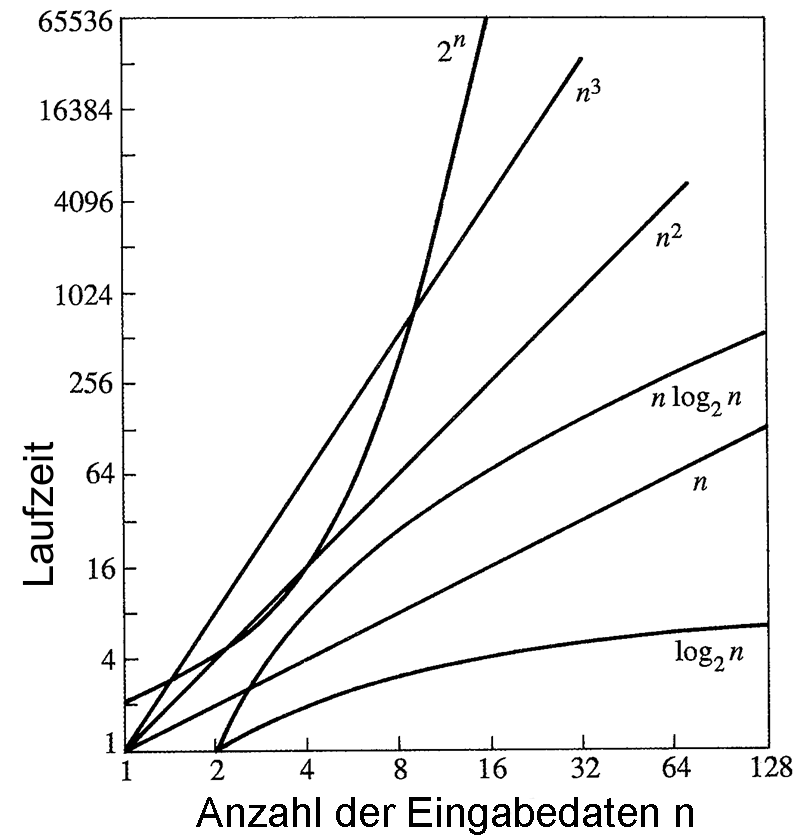
\includegraphics[scale=0.25]{graphics/09/laufzeiten.png}
		\end{center}
	\end{frame}
	
	
	\section{Aufgaben}
	\begin{frame}{Aufgaben}
		Bestimmen Sie die Laufzeit des Warshall-Algorithmus:
		
		\small
            \begin{algorithmic}
				\For{i}{0}{n-1}
					\For{j}{0}{n-1}
						\If{$i = j$}
							\State $W[i,j] \gets 1$;
						\Else
							\State $W[i,j] \gets A[i,j]$
						\EndIf
					\EndFor
				\EndFor
            \end{algorithmic}
            \begin{algorithmic}
				\For{k}{0}{n-1}
					\For{i}{0}{n-1}
						\For{j}{0}{n-1}
							\State $W[i , j ] \gets  max(W[i , j ]; min(W[i , k];W[k, j ]) )$
						\EndFor
					\EndFor
				\EndFor
            \end{algorithmic}
	\end{frame}
	
	
	\begin{frame}{Aufgaben}
		Zeigen oder widerlegen Sie:\\
		\vspace{10pt}
		\begin{itemize}
			\item $\frac{n^3+2n}{2n+1} \in 0(n^2)$
			\item $n! \in \Omega(n^2)$
		\end{itemize}
	\end{frame}
	
	
	\section{Fragen}
	\begin{frame} {Fragen}
		\begin{itemize}
			\item Fragen zum Stoff?
			\item Fragen zum n\"achsten \"Ubungsblatt?
			\item Generelle Fragen?
			\item Feedback?
		\end{itemize}
	\end{frame}

		
	\begin{frame} {Frohe Weihnachten}
		\begin{center}
			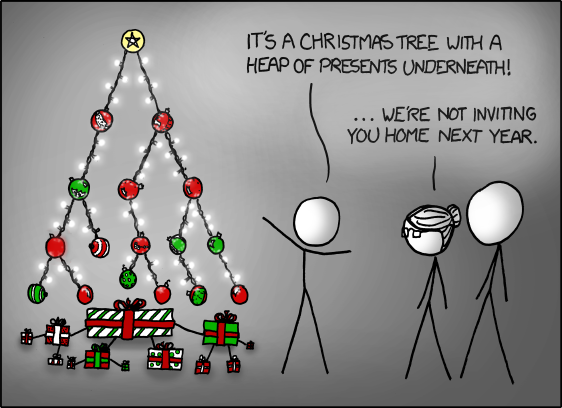
\includegraphics[scale=0.45]{graphics/eof9.png}\\
			\tiny $source: http://imgs.xkcd.com/comics/tree.png$
		\end{center}
	\end{frame}

\end{document}
